% status: 0
% chapter: Data

\title{ELK Stack}


\author{Karan Kamatgi}

\affiliation{%
  \institution{Indiana University Bloomington}
  \city{Bloomington} 
  \state{Indiana} 
  \postcode{47404}
}
\email{krkamatg@iu.edu.com}

\author{Gregor von Laszewski}
\affiliation{%
  \institution{Indiana University}
  \streetaddress{Smith Research Center}
  \city{Bloomington} 
  \state{IN} 
  \postcode{47408}
  \country{USA}}
\email{laszewski@gmail.com}


% The default list of authors is too long for headers}
\renewcommand{\shortauthors}{G. v. Laszewski}


\begin{abstract}

ELK acronyms for Elasticsearch, Logstash and Kibana which are a group of three 
open source products in the market. Elastic Search is a NoSQL database that 
uses and depends on Lucene search engine. Logstash is log pipelining application
 that takes inputs from different sources and performs various transformations 
 and finally exports data to various targets. Kibana is a data visualization 
 application that performs the data reporting and analytics on top of the 
 Elastic Search.

Although individually these open source projects have performed well but their 
potential contribution is realized when the three of them are combined together.
 These are usually combined and commonly used in log analysis, log extraction 
 and troubleshooting in IT environments where Logstash collects data and parses 
 logs and later Elastic Search indexes the data and stores the information in 
 the database. The visualization tool Kibana finally showcases the analyzed 
 data that provides information for further troubleshooting.

\end{abstract}

\keywords{hid-sp18-410,ELK,Elasticsearch,Logstash,Kibana,Log analytics
,data visualization}


\maketitle


\section{Introduction}

One of the most common problems in leading IT industries is handling data, 
analyzing data and troubleshooting production issues effectively and as early 
as possible to reduce the damage in production. Many organizations fail to 
understand the importance of data analysis which helps in understanding the 
problem that needs to be addressed. ELK is one of the many open source solutions
 that provide a suite of data analysis and visualization functions that can 
 perform the role of a powerful troubleshooting tool ~\cite{hid-sp18-410-elk-intro1}. 

 Google Analytics also serves the purpose of monitoring and data
 analysis which supports custom client and server events but working
 with custom events is a complex operation. It also lacks system
 performance counters, log aggregation and
 alerting~\cite{hid-sp18-410-elk-intro2}.  Datadog is another such
 tool that is targeted to administrators and people who needs high
 level understanding of servers and services. This happens to be the
 only tool that could monitor Solr and Dockr containers. This tool
 looks great but lacks log aggregation and also it is time consuming
 and requires complex work to get the SQL and IIS monitoring to
 actually run in production~\cite{hid-sp18-410-elk-intro2}.  Splunk's
 Enterprise software which more famous and leader in devops domain is
 seeing a sudden drop in the usage as the functionalities offered are
 not worth the prices.  ELK would not provide all the fancy features
 provided by splunk but is a simple, robust log analysis tool that
 costs very less compared to splunk~\cite {hid-sp18-410-elk-intro2}.



\section{Architecture}

Every organization has software applications that have tons and tons of logs 
being generated everyday or every hour depending on the needs of the 
application. Since Logging generates tremendous amount of data which stems more 
problems and challenges due to the varied and unstructured nature of logs. Some 
of the challenges include varied data log formats, different data log locations,
 different data date formats, decentralized data log creation and storage. 
 Searching files by keyword is not easy which is important feature in 
 troubleshooting. Hence ELK is a one stop solution to all the problems
 ~\cite{hid-sp18-410-elk-architecture}  
Figure~\ref{f:architecture} explains the ELK architecture and its workflow.

The first step in the process is to collect the logs and Logstash performs the 
job of collecting, filtering normalizing and sending the logs to a central 
location. Logstash uses some of the filtering techniques such as grok based on 
date, geoip and useragent.Next the structured and analyzed data is sent to 
forwarder that forwards the important deduced information to the remote endpoint
 usually ElasticSearch~\cite{hid-sp18-410-elk-architecture}
 Next ElasticSearch which is based on Lucene performs indexing and searching and
  finally stores the documents in JSON format. It provides simple and RESTFUL 
  API abstraction on top of lucene. Elasticsearch uses NoSQL database for 
  storing documents and uses queries for searching~\cite{hid-sp18-410-elk-architecture}.
This structured data is now sent to Kibana that provides a beautiful Graphical 
user interaction for the users to enter the reporting requirements which 
performs the final filtering of data based on the requirements and presents 
the data graphs, reports and information graphs that is very helpful for the 
users~\cite{hid-sp18-410-elk-architecture}

\begin{figure}[!ht]
  \centering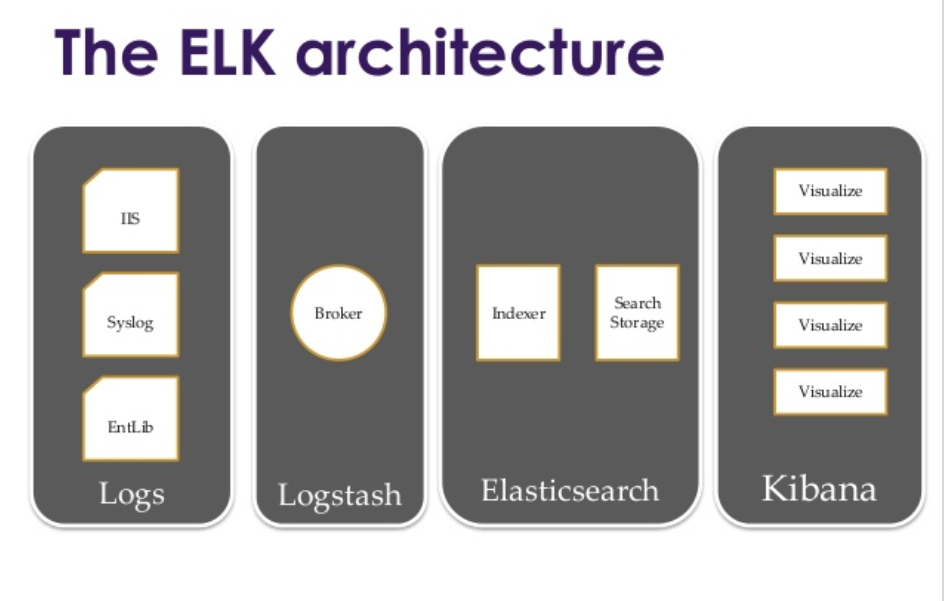
\includegraphics[width=\columnwidth]{image/ELK-Architecture.PNG}
  \caption{ELK Architecture~\cite{hid-sp18-410-elk-architecture-image}}
\label{f:architecture}
\end{figure}


\section{Components}


\subsection{Elasticsearch}

Elastics search open source tool is almost a real-time search engine which is 
highly scalable and flexible. Since it is based on Lucene 
(another open source software) makes indexing and searching easier. The main 
task of ElasticSearch is to provide an abstraction on top of the lucene which 
would perform the task of indexing and searching. This tool supports both 
vertical and horizontal scaling~\cite{hid-sp18-410-elk-components}  

Figure~\ref{f:elasticsearch} explains the master node and data node 
replication workflow.

\subsection{Logstash}

Logstash is a data collection pipeline tool that stands before Elasticsearch 
mainly to gather data inputs which are usually unstructured and unfiltered. 
Logstash supports a wide variety of data type and data sources. Next it uses 
various filtering techniques based on parameters like date, IP address and user 
agent.Logstash can magically collect these input data and provide the filtered 
and structured data within no time. This data is passed on to ElasticSearch 
~\cite{hid-sp18-410-elk-components}

Logstash pipeline is explained in Figure~\ref{f:logstash}


\subsection{Kibana}

Kibana is a data visualization platform that provides a beautiful dashboard for 
user to interact with ELK stack. Kibana visualizes the documents stored in NoSQL
 database of ElasticSearch along with timelines and Geospatial data that clearly
 indicates the various microservices that are being processed at various times.
  Kibana eases the task for developers by creating and saving graphs that best 
suit the needs of the particular application
~\cite{hid-sp18-410-elk-components}

Kibana workflow is better explained at Figure~\ref{f:kibana}

\begin{figure}[!ht]
  \centering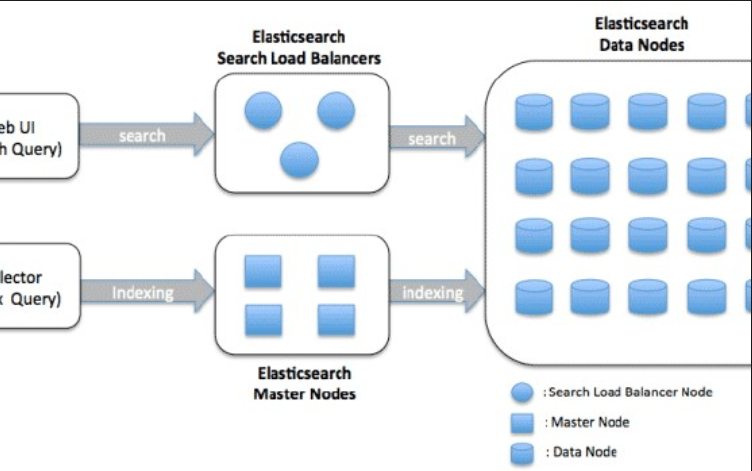
\includegraphics[width=\columnwidth]{image/elasticsearch}
  \caption{Elastic Search tool~\cite{hid-sp18-410-elk-comp1}}
\label{f:elasticsearch}
\end{figure}

\begin{figure}[!ht]
  \centering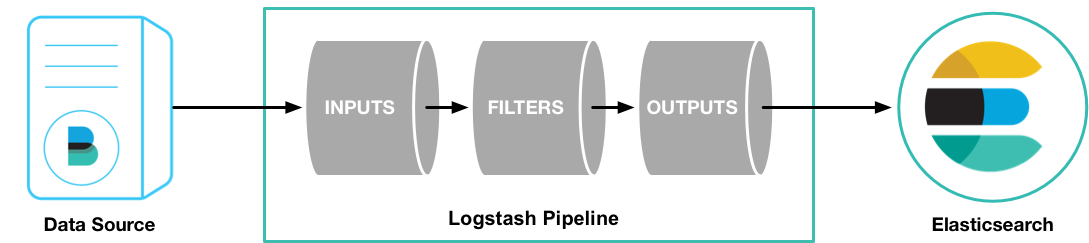
\includegraphics[width=\columnwidth]{image/logstash.png}
  \caption{Logstash~\cite{hid-sp18-410-elk-comp2}}\label{f:logstash}
\end{figure}

\begin{figure}[!ht]
  \centering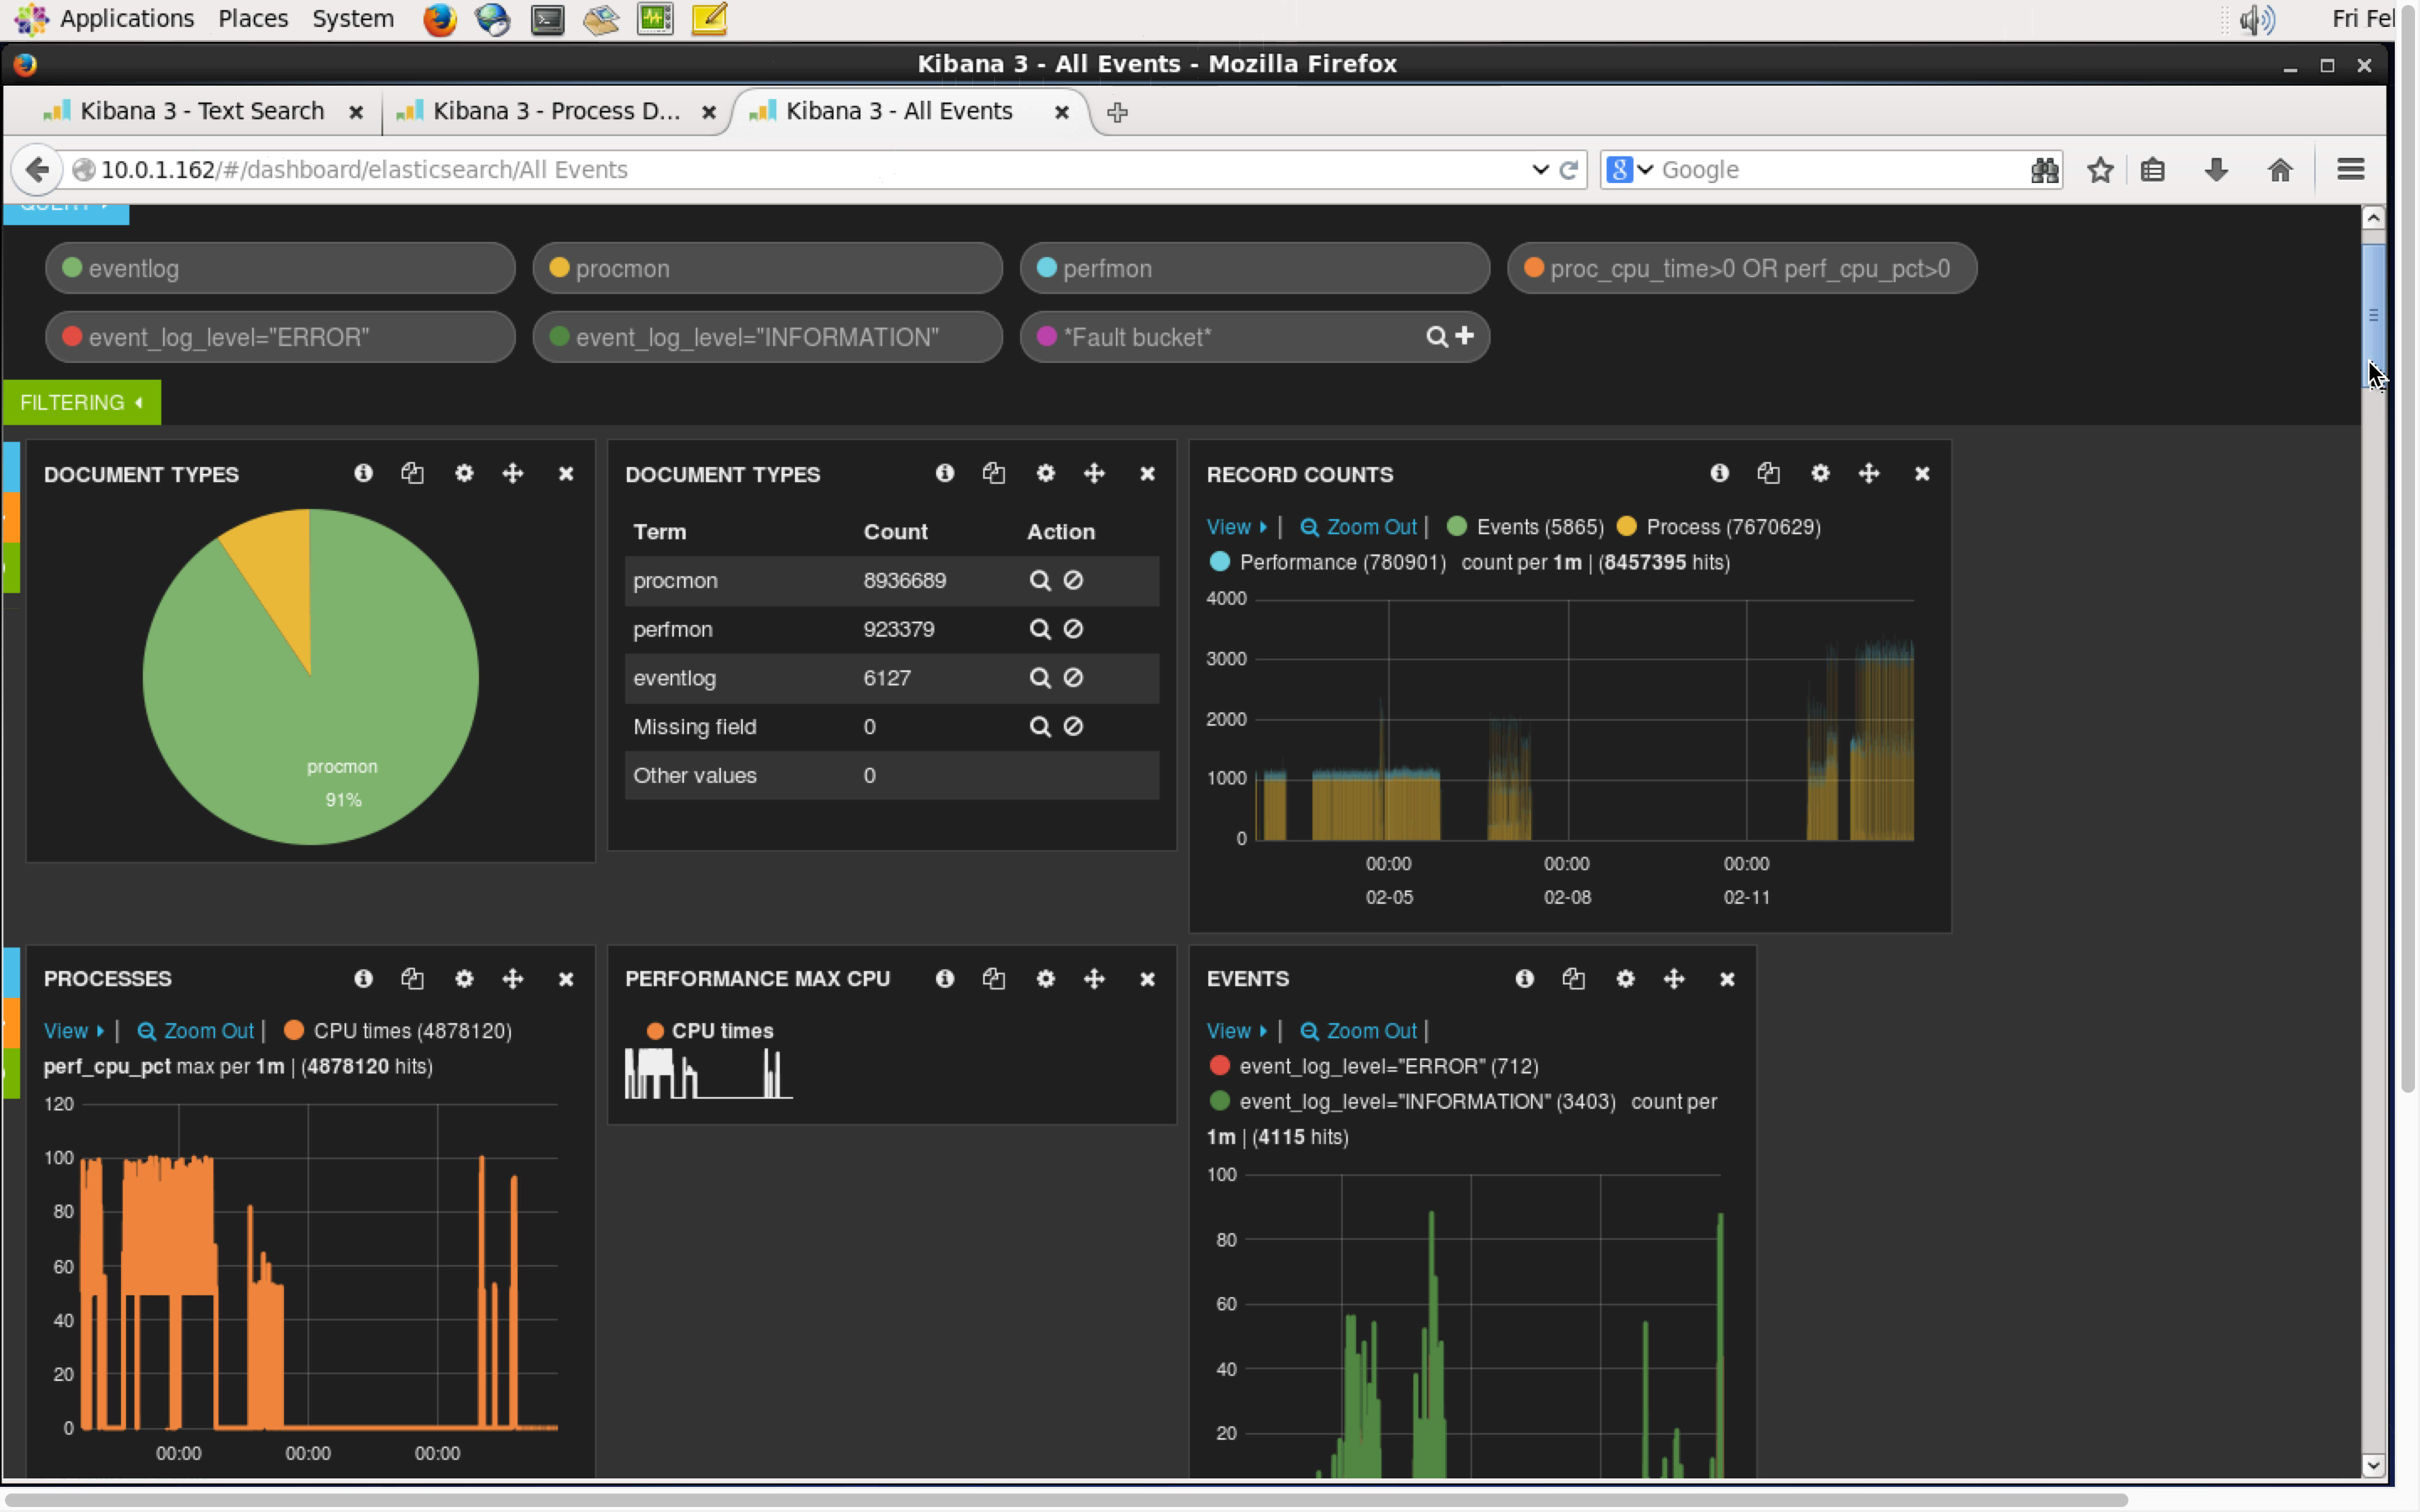
\includegraphics[width=\columnwidth]{image/kibana.png}
  \caption{Kibana~\cite{hid-sp18-410-elk-comp3}}\label{f:kibana}
\end{figure}


\section{Use case}

Due to the flexible and scalable nature of ELK stack there are always 
newer uses cases emerging as more and more enhancements are added to existing 
components. Some of the top use cases include Log analytics, web search, 
product search, metric analytics and website search. 

\subsection{Log and security analytics}

The traditional infrastructure of an application includes web servers, database 
servers, application servers and message brokers. It is practically impossible 
to log into each individual server and inspect unstructured log files. ELK 
provides complete tool set solution that collect, analyze, visualize and report 
errors~\cite{hid-sp18-410-elk-usecase}.  

\subsection{Product Search}

searching for most relevant products from hundreds, thousands and millions of 
other products. This is comparable to the problem of e-commerce websites that 
sell huge number of products by various vendors and sellers.
~\cite{hid-sp18-410-elk-usecase}.

\subsection{Metric analytics}

Since Elastic search provides powerful aggregation API which embraces excellent 
analytics capabilities. Elastic search and Kibana supports slicing and dicing 
of metric data to extract deep information out of them thus making ELK powerful 
tool for handling metric analytics~\cite{hid-sp18-410-elk-usecase}. 


\subsection{Web search and website search}

elastic search can be leveraged as search engine for your website and also could
 be used as key-word search for entire application data. Github, Wikipedia and 
 other platforms increase their search performance using Elasticsearch. ELK also
  provides excellent support for building content aggregation frameworks
  ~\cite{hid-sp18-410-elk-usecase}  




\section{Conclusion}

With the increasing number of organization trying to develop applications 
involving huge data often times run into various challenges such as efficient 
data reporting, effective log analytics for trouble shooting production issues, 
content delivery and application aggregation, monitoring and indexing.

Since ELK stack has three different components working together in a pipeline 
has proven to be extremely versatile and the ability to enhance the 
technologies, scalability and flexibility are biggest features provided by ELK. 
This solution just does not provide another database to store your data but 
rather provide smart and effective way to solve the problem with increasing 
capability to enhance itself to the business needs.

ELK strives hard to offer set of utilities and tools each one of them existing 
for a definitive reason. If each of these utilities and tools are combined which
would create search and log analytics platform for any kind of business 
architecture.Every IT department of any organization aspire to have a 
centralized logging mechanism that could easily and effectively identify server
problems that reduces the production impact. All the clients could leverage the
various factored reporting graphical user interaction tool called Kibana that 
provides a beautiful dashboard for data visaualization and data reporting.

There is a lot of scope for improvements with respect to security and also the 
out of the box tool lacks monitoring, which could have been incorporated thus 
providing it as a service. More configurations and settings needs to be carried 
on the client side could be offloaded to the server side depending on the 
application and its usage. 



\begin{acks}

  The authors would like to thank Dr.~Gregor~von~Laszewski for his
  support and suggestions to write this paper.

\end{acks}

\bibliographystyle{ACM-Reference-Format}
\bibliography{report} 

